%!TEX root = ../main.tex

\chapter{Algoritmo di backpropagation}
\label{cha:algoritmo_di_back_propagation}

Negli anni settanta c'è stato un generale disinteresse nei confronti delle reti neurali, a causa della scoperta delle limitazioni dei percettroni a singolo strato e dell'incapacità di addestrare le più potenti reti multistrato.

Il problema incontrato era il seguente: volendo adottare un meccanismo di aggiornamento dei pesi simile a quello nelle reti single layer, in cui l'errore è calcolato come differenza tra l'uscita desiderata e l'uscita effettiva di ciascun neurone, si era in grado di aggiornare solo i pesi relativi ai neuroni di uscita; infatti, mentre per lo strato di uscita si conosce l'output desiderato, che viene dato come secondo elemento delle coppie che costituiscono il training set, non si sa nulla a riguardo dell'uscita desiderata per i neuroni nascosti.

Il problema è stato risolto da D. E. Rumelhart, G. E. Hinton e R. J. Williams, che nel 1986 hanno introdotto l'\textbf{algoritmo di backpropagation} per  l'addestramento di reti neurali \textbf{feedforward multistrato}. L'algoritmo prevede di calcolare l'errore commesso da un neurone dell'ultimo strato nascosto propagando all'indietro l'errore calcolato sui neuroni di uscita collegati ad esso; lo stesso procedimento è poi ripetuto per tutti i neuroni del penultimo strato nascosto e così via.

Requisito fondamentale per l'utilizzo dell'algoritmo è la \textbf{derivabilità} della funzione di attivazione dei neuroni, in quanto l'algoritmo è basato sul metodo della \textbf{discesa del gradiente} per la minimizzazione dell'\textbf{errore} commesso dalla rete.

\section{Metodo di discesa del gradiente}
\label{sec:metodo_di_discesa_del_gradiente}

Il \textbf{gradiente} di una funzione $f$, indicato con $\nabla f$, è il vettore che ha come componenti le derivate parziali della funzione.
\begin{displaymath}
	\nabla f(\vec{x}) = \left( \frac{\partial f(\vec{x})}{\partial x_1}, \frac{\partial f(\vec{x})}{\partial x_2}, \dots, \frac{\partial f(\vec{x})}{\partial x_n} \right)
\end{displaymath}
La discesa del gradiente è una tecnica di ottimizzazione di tipo \textbf{locale}: consiste nel valutare, inizialmente in un punto scelto in maniera casuale, sia la funzione stessa sia il suo gradiente.

Dal momento che quest'ultimo indica la direzione di massima crescita della funzione, si considerano i passi proporzionali al \textbf{negativo} del gradiente della funzione nel punto corrente e la si valuta nel nuovo punto. La procedura viene arrestata quando, in seguito ad uno spostamento, il valore della funzione obiettivo aumenta anziché diminuire.\footnote{Quando si è interessati alla ricerca di un punto di massimo si prendono passi proporzionali al positivo del gradiente: in tal caso la procedura è nota come \textbf{ascesa del gradiente}.}

\section{Apprendimento supervisionato}
\label{sec:apprendimento_supervisionato}

L'algoritmo di backpropagation è un algoritmo di \textbf{apprendimento supervisionato}, ovvero richiede un \textbf{training set} $L$ del tipo
\begin{displaymath}
	L = \{(\vec{x}^1, \vec{y}^1), \dots, (\vec{x}^P, \vec{y}^P) \}
\end{displaymath}
dove
\begin{itemize}
	\item $\vec{x}^\mu$ ($\mu=1, \dots, P$) è il vettore di input;
	\item $\vec{y}^\mu$ ($\mu=1, \dots, P$) è il vettore dell'output desiderato.
\end{itemize}
I pesi vengono tipicamente inizializzati in maniera casuale all'inizio dell'addestramento, poi si presentano, uno alla volta, gli esempi del training set: per ciascuno si calcola l'errore commesso dalla rete, ovvero la differenza tra l'uscita desiderata e l'uscita effettiva della rete, che viene utilizzato per aggiustare i pesi.

Il processo viene ripetuto ripresentando alla rete, in ordine casuale, tutti gli esempi del training set finchè l'errore medio risulta inferiore ad una soglia prestabilita.

Formalmente la fase di apprendimento consiste nel trovare una configurazione di pesi tale da minimizzare la \textbf{funzione di errore}
\begin{align*}
	E(\vec{w}) &= \frac{1}{2} \sum_{\mu=1}^P \| \vec{y}^\mu- \vec{out}^\mu (\vec{w}) \|^2 \\
	&= \frac{1}{2} \sum_{\mu=1}^P \sum_{k=1}^n \left(y_k^\mu - out_k^\mu (\vec{w})\right)^2
\end{align*}
dove $\vec{out}^\mu$ è l'output fornito dalla rete quando $\vec{x}^\mu$ è dato in input.

Al termine della fase di addestramento, la rete viene testata controllandone il comportamento su un insieme di dati, detto \textbf{test set}, costituito da esempi non utilizzati durante la fase di training. La fase di test ha quindi lo scopo di valutare la capacità di \textbf{generalizzazione} della rete neurale: si dice che la rete ha imparato se è in grado di fornire risposte anche per ingressi che non le sono mai stati presentati durante la fase di addestramento.

Ovviamente le prestazioni di una rete neurale dipendono fortemente dall'insieme di esempi scelti per l'addestramento: essi devono essere rappresentativi della realtà che la rete deve apprendere e in cui verrà utilizzata. L'apprendimento è infatti un processo ad hoc dipendente dallo specifico problema trattato.

\section{Propagazione dell'errore}
\label{sec:back_propagation}

L'algoritmo di backpropagation può essere diviso in due passi:
\begin{itemize}
	\item \textbf{forward pass}: l'input dato alla rete è propagato in avanti, strato dopo strato, fino al livello di uscita, dove viene calcolato l'errore commesso $E(\vec{w})$;
	\item \textbf{backward pass}: l'errore è propagato all'indietro e i pesi sono aggiornati in maniera appropriata.
\end{itemize}
Consideriamo la rete neurale in figura \ref{fig:backpro} per derivare le formule di aggiornamento dei pesi: l'algoritmo può chiaramente essere utilizzato su reti di dimensione arbitraria.
\begin{figure}[h!]
	\centering
	\begin{tikzpicture}[->,shorten >=2pt, shorten <= 2pt, auto, node distance=\layersep]
		\def\nodesep{-2cm}
		\def\layersep{4cm}
		% Draw the input layer nodes
		\foreach \name / \y in {1,...,4}
		\node[input neuron, pin={left:$x_\y$}] (I-\name) at (0, \nodesep * \y) {};

		% Draw the hidden layer nodes
		\foreach \name / \y in {1,...,3}   
		\node[hidden neuron, pin={[pin edge={->}]above:$V_\y$}] (H-\name) at (\layersep, \nodesep * \y - 1 cm) {};
            
		% Draw the output layer nodes
		\foreach \name / \y in {1,...,2}   
		\node[output neuron, pin={[pin edge={->}]right:$O_\y$}] (O-\name) at (2*\layersep, \nodesep * \y - 2cm) {};

		% Connect every node in the input layer with every node in the hidden layer.
		\foreach \source in {1,...,4}
		\foreach \dest in {1,...,3}
		\path (I-\source) edge (H-\dest);

		% Error edges.
		\foreach \source in {1,...,4}
		\foreach \dest in {1,...,3}
		\path (H-\dest) edge[dashed, color=red, transform canvas={yshift=1mm}] (I-\source);

		\foreach \source in {1,...,3}
		\foreach \dest in {1,...,2}
		\path (O-\dest) edge[dashed, color=red, transform canvas={yshift=1mm}] (H-\source);


		\path (I-1) edge[above] node {$w_{11}$} (H-1);
		\path (I-4) edge[below] node {$w_{34}$} (H-3);
		% Connect every node in the hidden layer with every node in the output layer.
		\foreach \source in {1,...,3}
		\foreach \dest in {1,...,2}
		\path (H-\source) edge (O-\dest);


		\path (H-1) edge[above] node {$W_{11}$} (O-1);
		\path (H-3) edge[below] node {$W_{23}$} (O-2);
        
		% Annotate the layers
		\node[annot,above of=H-1, node distance=2cm] (hl) {Hidden layer};
		\node[annot,left of=hl] {Input layer};
		\node[annot,right of=hl] {Output layer};
        
		\node at (-1.3, - 9) {$x_k$};
		\node at (2, - 9) {$w_{jk}$};
		\node at (4, - 9) {$V_j$};
		\node at (6, - 9) {$W_{ij}$};
		\node at (9.3, - 9) {$O_i$};
        
	\end{tikzpicture}
	\caption[Schema back-propagation]{Schema back-propagation: le linee nere indicano il segnale propagato in avanti, mentre quelle rosse indicano l'errore propagato all'indietro.}
	\label{fig:backpro}
\end{figure}

\noindent Dato un pattern $\mu$, l'unità nascosta $j$ riceve un input netto dato da
\begin{displaymath}
	h_j^\mu = \sum_k w_{jk} x^\mu_k
\end{displaymath}
e produce come output
\begin{displaymath}
	V_j^\mu = g(h_j^\mu) = g\left(\sum_k w_{jk} x^\mu_k \right)
\end{displaymath}
dove $g$ è la funzione di attivazione. In modo del tutto analogo si possono definire input e output dei neuroni dello strato di uscita.

I pesi sono aggiornati nella direzione opposta rispetto al gradiente, in quanto siamo interessati a minimizzare la funzione di errore, in accordo alla seguente formula (dove $t$ è il numero di iterazioni):
\begin{displaymath}
	\vec{w}^{(t+1)} = \vec{w}^{(t)} - \eta \nabla (E(\vec{w}^{(t)}))
\end{displaymath}
Il parametro $\eta$, noto come \textbf{fattore di apprendimento}, ha una forte influenza sul comportamento dell'algoritmo (velocità di convergenza, oscillazioni, ecc.).
\begin{figure}[h!]
	\centering
	\begin{tikzpicture}
		\node[draw,circle,inner sep=1pt,fill] (1) at (0, 0) {};
		\node[above right=1mm of 1] {$\vec{w}^{(t)}$};
		\node[draw,circle,inner sep=1pt,fill] (2) at (2, -1) {};
		\node[above right=1mm of 2] {$\vec{w}^{(t+1)}$};
		\node (3) at (4, -2) {};
		\draw[->] (2) -- (3);
		\node[below=0.1mm of 3] {$-\nabla (E(\vec{w}^{(t)}))$};
		\path (1) edge[very thick, below] node {$\eta$} (2);
	\end{tikzpicture}
	\caption{Direzione di aggiornamento dei pesi.}
\end{figure}

\subsection{Aggiornamento pesi strato nascosto-output}
\label{sub:aggiornamento_pesi_strato_nascosto_output}

Deriviamo ora la formula per il calcolo della variazione di peso sinaptico tra il neurone $j$ dello strato nascosto e il neurone $i$ dello strato di output.
\begin{align*}
	\Delta W_{ij} &= - \eta \frac{\partial E}{\partial W_{ij}} \\
	&= \eta \sum_\mu \sum_k (y_k^\mu -O_k^\mu) \frac{\partial O_k^\mu}{\partial W_{ij}} \\
	\intertext{Per $k\neq i$, $O_k$ non dipende da $W_{ij}$, quindi la derivata è 0.}
	&= \eta \sum_\mu (y_i^\mu - O_i^\mu) \frac{\partial O_i^\mu}{\partial W_{ij}} \\
	&= \eta \sum_\mu (y_i^\mu - O_i^\mu) g'(h_i^\mu) \frac{\partial h_i^\mu}{\partial{W_{ij}}}
\end{align*}
Calcoliamo ora $\partial h_i^\mu / \partial W_{ij}$:
\begin{align*}
	\frac{\partial h_i^\mu}{\partial{W_{ij}}} &= \frac{\partial}{\partial{W_{ij}}} \sum_l V_l^\mu W_{il} \\
	&= \frac{\partial}{\partial{W_{ij}}} V_j^\mu W_{ij} = V_j^\mu
\end{align*}
Quindi si ha
\begin{align*}
	\Delta W_{ij} = \eta \sum_\mu (y_i^\mu - O_i^\mu) g'(h_i^\mu) V_j^\mu = \eta \sum_\mu \delta^\mu_i V^\mu_j
\end{align*}
dove
\begin{align*}
	\delta^\mu_i = (y^\mu_i - O^\mu_i) g'(h^\mu_i)
\end{align*}
è l'errore del neurone $i$-esimo ed è noto come \textbf{gradiente locale}.

\subsection{Aggiornamento pesi strato input-nascosto}\label{sub:aggiornamento_pesi_strato_input_nascosto}

Passiamo ora al calcolo della variazione di peso sinaptico tra il neurone nascosto $j$ e l'unità di input $k$.
\begin{align*}
	\Delta w_{jk} &= - \eta \frac{\partial E}{\partial w_{jk}} \\
	&= \eta \sum_\mu \sum_i (y^\mu_i - O^\mu_i) \frac{\partial O^\mu_i}{\partial w_{jk}} \\
	&= \eta \sum_\mu \sum_i (y^\mu_i - O^\mu_i) g'(h^\mu_i) \frac{\partial h^\mu_i}{\partial w_{jk}}
\end{align*}
In questo caso la seconda sommatoria rimane, in quanto l'output di ogni neurone nello strato di uscita dipende indirettamente da $w_{jk}$.

Calcoliamo ora $\partial h^\mu_i / \partial w_{jk}$:
\begin{align*}
	\frac{\partial h^\mu_i}{\partial w_{jk}} &= \sum_l W_{il} \frac{\partial V_l^\mu}{\partial w_{jk}} \\
	\intertext{Per $l\neq j$, $V_l$ non dipende da $w_{jk}$.}
	&= W_{ij} \frac{\partial V_j^\mu}{\partial w_{jk}} \\
	&= W_{ij} g'(h^\mu_j) \frac{\partial h^\mu_j}{\partial w_{jk}}
\end{align*}
La derivata $\partial h^\mu_j / \partial w_{jk}$ è:
\begin{align*}
	\frac{\partial h^\mu_j}{\partial w_{jk}} 
	&= \frac{\partial}{\partial w_{jk}} \sum_m w_{jm} x^\mu_m \\
	&= \frac{\partial}{\partial w_{jk}} w_{jk} x^\mu_k\\
	&= x^\mu_k
\end{align*}
Riassumendo abbiamo
\begin{align*}
	\Delta w_{jk} &= \eta \sum_\mu \sum_i (y_i^\mu - O^\mu_i) g'(h^\mu_i) W_{ij} g'(h_j^\mu) x^\mu_k\\
	&= \eta \sum_\mu \sum_i \delta_i^\mu W_{ij} g'(h_j^\mu) x^\mu_k \\
	&= \eta \sum_\mu \delta_j^\mu x^\mu_k
\end{align*}
dove
\begin{displaymath}
	\delta_j^\mu = g'(h_j^\mu) \sum_i \delta^\mu_i W_{ij}
\end{displaymath}
è il gradiente locale del neurone nascosto $j$ e la sommatoria rappresenta l'errore medio sullo strato di output causato dal neurone $j$ dello strato nascosto.

\subsection{In sintesi}
\label{ssub:in_generale}

In generale, per l'aggiornamento dei pesi non sono necessarie informazioni globali, ma solo \textbf{locali}. La variazione di peso sinaptico tra un neurone $p$ e $q$, in accordo alle formule derivate nelle sezioni precedenti, è dato da
\begin{displaymath}
	\Delta w_{pq} = \eta \sum_\mu \delta^\mu_p V^\mu_q
\end{displaymath}
dove
\begin{displaymath}
	\delta_p^\mu = \begin{cases}
		(y^\mu_p - O^\mu_p) g'(h^\mu_p) & \text{se $p$ è un neurone di output} \\
		\displaystyle g'(h_p^\mu) \sum_i \delta^\mu_i W_{ip} &\text{altrimenti}
	\end{cases}
\end{displaymath}
Questo modello prende il nome di apprendimento \textbf{offline}, in quanto calcola la variazione di peso usando contemporaneamente tutti gli esempi dell'insieme di addestramento.

Un modello più coerente con quello biologico è detto apprendimento \textbf{online}, dove la rete apprende un esempio per volta:
\begin{displaymath}
	\Delta w_{pq} = \eta \delta^\mu_p V^\mu_q
\end{displaymath}

\section{L'algoritmo di backpropagation}
\label{sec:l'algoritmo}

Consideriamo una rete con $M$ strati ed indichiamo
\begin{itemize}
	\item $V^m_i$: output della $i$-esima unità del livello $m$;
	\item $w^m_{ij}$: peso della connessione tra il $j$-esimo neurone dello strato $m-1$ e l'$i$-esimo neurone dello strato $m$. 
\end{itemize}
con $m = 0, \dots, M$. L'algoritmo è il seguente:
\begin{algorithmic}[1]
	\State Inizializzazione dei pesi a (piccoli) valori casuali;
	\State Scelta di un pattern $\vec{x}^\mu$ da inserire allo strato input:
	\begin{align*}
		V^0_k = x^\mu_k \qquad \forall k
	\end{align*}
	\State Propagazione del segnale in avanti ($m = 1, \dots, M$):
	\begin{align*}
		V^m_i = g(h_i^m) = g\left(\sum_j w_{ij}^m V_j^{m-1}\right)
	\end{align*}
	\State Calcolo degli errori $\delta$ dello strato di output:
	\begin{align*}
		\delta^M_i = (y_i - V^M_i) \, g'(h^M_i)
	\end{align*}
	\State Calcolo degli errori $\delta$ per gli strati precedenti ($m = M, \dots, 2)$:
	\begin{align*}
		\delta^{m-1}_i = g'\left(h^{m-1}_i\right) \, \sum_j \delta^m_j \, w_{ji}^m
	\end{align*}
	\State Aggiornamento dei pesi ($m = 1, \dots, M$):
	\begin{align*}
		w^{(t + 1)}_{ij} = w^{(t)}_{ij} + \Delta w_{ij} \qquad \text{dove } \Delta w_{ij} = \eta \delta_i^m V_j^{m-1} 
	\end{align*}
	\State Torna al passo 2 fino alla convergenza.
\end{algorithmic}
L'algoritmo si può terminare quando $\|\vec{w}^{(t+1)} - \vec{w}^{(t)}\| < \epsilon$ oppure dopo un certo numero di epoche\footnote{Un'\textbf{epoca} è un ciclo di presentazione di tutti gli elementi del training set.} se la condizione precedente non è rispettata.

\section{Il momento}
\label{sub:il_momento}

La scelta del fattore di apprendimento $\eta$ influenza pesantemente il comportamento dell'algoritmo: se scegliamo valori troppo piccoli, la convergenza sarà lenta, se scegliamo valori troppo grandi si rischia di avere un comportamento oscillatorio.

Un metodo semplice per incrementare $\eta$ senza il rischio di rendere l'algoritmo instabile consiste nel modificare la regola di aggiornamento inserendo un nuovo termine, il \textbf{momento}, proporzionale alla precedente variazione dei pesi. La regola di aggiornamento diventa
\begin{displaymath}
	\Delta w_{pq}^{(t + 1)} = \alpha \Delta w_{pq}^{(t)} - \eta \frac{\partial E}{\partial w_{pq}}
\end{displaymath}
dove $\alpha$ è un numero positivo a scelta preferibilmente compreso in $[0,1)$. In generale si utilizzano $\alpha = 0.9$ e $\eta = 0.5$.

L'utilizzo del momento ha l'effetto di incrementare o decrementare l'ampiezza di aggiornamento in modo tale da \textbf{accellerare} nelle discese o \textbf{stabilizzare} l'algoritmo in caso di oscillazioni. Il suo utilizzo, inoltre, ha il vantaggio di \textbf{prevenire} (non con certezza) che il processo di apprendimento incappi in minimi locali della funzione d'errore.

\begin{figure}[h!]
	\centering
	\subfigure[Assenza di momento $\alpha=0$]{
	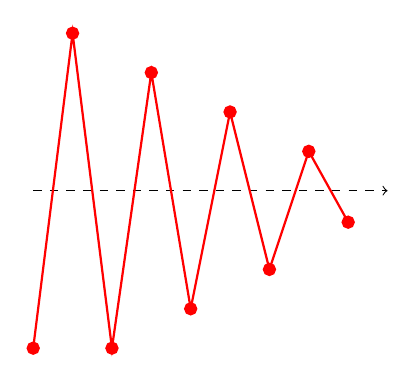
\begin{tikzpicture}
		\draw[->, dashed] (-2,0) -- (2.5,0);
		\draw[thick, color=red] plot [mark=*,red, tension=1.5] coordinates{
		(-2,-2) (-1.5, 2) (-1, -2) (-0.5, 1.5) (0, -1.5) (0.5, 1) (1, -1) (1.5, 0.5) (2, -0.4)};
	\end{tikzpicture}
	}
	\qquad
	\subfigure[Con momento $\alpha=0.5$]{
	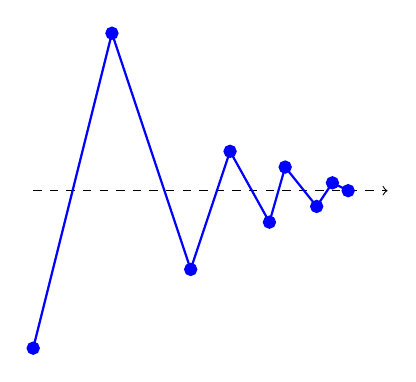
\begin{tikzpicture}
		\draw[->, dashed] (-2,0) -- (2.5,0);
		\draw[thick, color=blue] plot [mark=*,blue, tension=1.5] coordinates{
		(-2,-2) (-1, 2) (0, -1) (0.5, 0.5) (1, -0.4) (1.2, 0.3) (1.6, -0.2) (1.8, 0.1) (2, 0)};
	\end{tikzpicture}
	}
	\caption{Momento e discesa del gradiente su una semplice superficie.}
\end{figure}

\section{Problema del minimo locale}
\label{sec:problema_del_minimo_locale}

L'algoritmo di backpropagation non è sempre in grado di trovare il \textbf{minimo globale}. Il problema risiede nell'esistenza di \emph{buoni} e \emph{cattivi} punti di minimo.

\begin{figure}[h!]
	\centering
	\begin{tikzpicture}
		% Axes
		\draw [->, name path=x] (-1,0) -- (12,0) node [right] {$x$};
		\draw [->] (0,-1) -- (0,6) node [above] {$y$};
		% Origin
		\node at (0,0) [below left] {$0$};
		% Points
		\coordinate (start) at (0,5);
		\coordinate (c1) at (2,2);
		\coordinate (c2) at (4,3);
		\coordinate (c3) at (6,1);
		\coordinate (c4) at (8,5);
		\coordinate (c5) at (10,4);
		\coordinate (end) at (12,5);
		% show the points
		%   \foreach \n in {start,c1,c2,c3,end} \fill [blue] (\n)
		%       circle (1pt) node [below] {\n};
		% join the coordinates
		\draw [thick,name path=curve] (start) to[out=0,in=180] (c1) to[out=0,in=180]
		(c2) to[out=0,in=180] (c3) to[out=0,in=180] (c4) to[out=0,in=180] (c5) to[out=0,in=180] (end);
		% add tangets and dashed lines
		\foreach \c / \name in {1/buon minimo locale,3/minimo globale, 5/pessimo minimo locale} {
		\draw [dashed] let \p1=(c\c) in (c\c) -- (\x1,0) node [below] {\name};
		\draw ($(c\c)-(0.75,0)$) -- ($(c\c)+(0.75,0)$) node [midway,above=4mm] {};
		}
	\end{tikzpicture}
	\caption{Rappresentazione del problema del minimo locale.}
\end{figure}

Per evitare il problema è importante scegliere una configurazione iniziale adeguata dei pesi: se essi sono troppo elevati la derivata della funzione $g$ sarà vicina a zero e di conseguenza la variazione dei pesi sarà piccola, aumentando così il rischio di incappare in un minimo locale. Nella pratica si utilizza la seguente euristica per impostare i pesi iniziali:
\begin{displaymath}
	w_{ij} = \frac{1}{\sqrt{k_i}}
\end{displaymath}
dove $k_i$ è il numero di unità entranti nell'unità $i$.
